\documentclass[a4paper]{scrartcl}
\usepackage[cm]{fullpage}
\usepackage{amsmath, amssymb, esint}
\usepackage{siunitx}
\usepackage{graphicx, caption, subcaption}

\begin{document}

\title{PHYS3111: Assignment 1}
\author{ \\ \\ }
\date{2017-03-16}
\maketitle

\section{Consider the \(\delta\)-function potential, \(U(x) = g \delta(x)\). Solve the scattering problem and hence find the transmission and reflection amplitudes.}
Consider the time-independent Schr\"odinger equation:
\[-\frac{\hbar^2}{2 m} \frac{\mathrm{d}^2 \psi}{\mathrm{d} x^2} + U \psi = E \psi\]

Since our potential is discontinuous, we expect to find a discontinuity in the derivative of our wavefunction (but the wavefunction itself is still continuous). To do this, we can integrate the Schr\"odinger equation around the discontinuity, and solve for \(\frac{\mathrm{d} \psi}{\mathrm{d} x} \big|_{-\varepsilon}^{\varepsilon}\), with \(\varepsilon \to 0\):
\[\int_{-\varepsilon}^{\varepsilon} -\frac{\hbar^2}{2 m} \frac{\mathrm{d}^2 \psi}{\mathrm{d} x^2} + g \delta(x) \psi \:\mathrm{d} x = \int_{-\varepsilon}^{\varepsilon} E \psi \:\mathrm{d} x\]
\[-\frac{\hbar^2}{2 m} \frac{\mathrm{d} \psi}{\mathrm{d} x} \bigg|_{-\varepsilon}^{\varepsilon} + g \theta(x) \psi(0) \bigg|_{-\varepsilon}^{\varepsilon} = 0\]
\[\therefore \lim_{\varepsilon \to 0} \frac{\mathrm{d} \psi}{\mathrm{d} x} \bigg|_{-\varepsilon}^{\varepsilon} = \frac{2 m g}{\hbar^2} \psi(0)\]

For the scattering problem, \(E > 0\). Considering the left and right of the \(\delta\)-potential separately, we obtain the following solutions to the Schr\"odinger equation:
\begin{align*}
    \psi(x < 0) &= A e^{i k x} + B e^{-i k x} \\
    \psi(x > 0) &= C e^{i k x} + D e^{-i k x} \\
    k &= \sqrt{\frac{2 m E}{\hbar^2}}
\end{align*}

Applying our continuity condition on wavefunctions:
\begin{align*}
    \lim_{x \to 0^+} \psi &= \lim_{x \to 0^-} \psi \\
    A + B &= C + D
\end{align*}
\begin{align*}
    \lim_{x \to 0^+} \frac{\mathrm{d} \psi}{\mathrm{d} x} &= \lim_{x \to 0^-} \frac{\mathrm{d} \psi}{\mathrm{d} x} + \frac{2 m g}{\hbar^2} \psi(0) \\
    i A k - i B k &= i C k - i D k + \frac{2 m g}{\hbar^2} (C + D) \\
    A - B &= C - D + \frac{2 m g}{i \hbar^2 k} (C + D)
\end{align*}

We can interpret the constants \(A\), \(B\), \(C\) and \(D\) as the amplitudes of the waves traveling to the right (\(A\)) and left (\(B\)), left of the potential; and right (\(C\)) and left (\(D\)), right of the potential.

Consider an incident wave to the left of the potential, so \(A = 1\) and \(D = 0\), we can then solve for \(B\) and \(C\) to find the reflected and transmitted amplitudes, respectively:
\[\begin{cases}
    1 + B = C \\
    1 - B = C + 2 \alpha C
\end{cases}\]
\begin{align*}
    \therefore B &= \frac{-\alpha}{1 + \alpha} \\
    C &= \frac{1}{1 + \alpha} \\
    \alpha &= \frac{m g}{i \hbar^2 k}
\end{align*}

The corresponding \emph{intensities} are would then be \(R = |B|^2\) and \(T = |C|^2\).

\section{Sketch the probability densities of the wavefunctions \(\psi = \frac{1}{\sqrt{2}} (Y_{0, 0} + Y_{1, 0})\) and \(\psi = \frac{1}{\sqrt{2}} (Y_{0, 0} + Y_{2, 0})\) versus \(\theta\). Comment on the qualitative differences between the results.}
\begin{figure}[h]
    \centering
    \begin{subfigure}[b]{0.45\textwidth}
        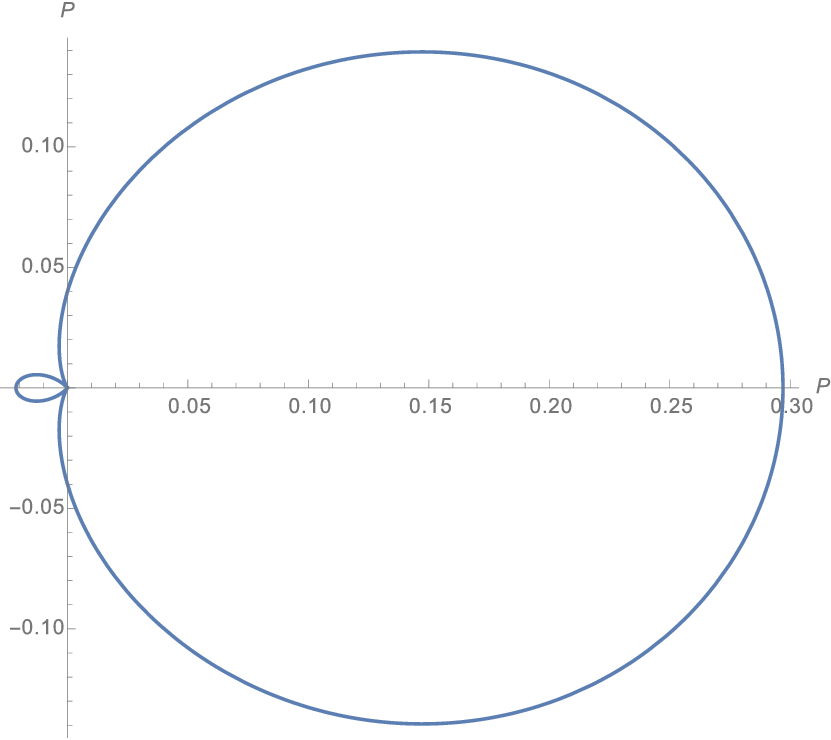
\includegraphics[width = \textwidth]{orbital-sp-polar.png}
    \end{subfigure}
    ~
    \begin{subfigure}[b]{0.45\textwidth}
        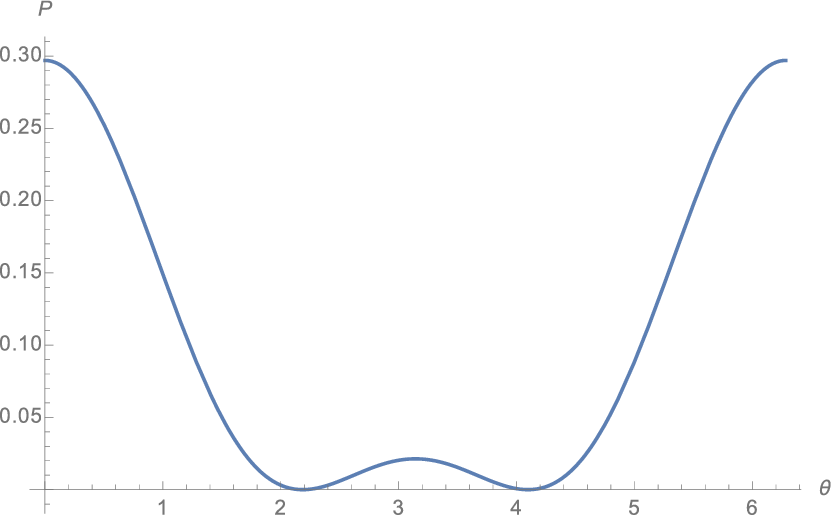
\includegraphics[width = \textwidth]{orbital-sp.png}
    \end{subfigure}
    \caption{Polar and non-polar plots of hybrid sp orbital probability densities}
    \label{fig:orbital-sp}
\end{figure}
\begin{figure}[h]
    \centering
    \begin{subfigure}[b]{0.45\textwidth}
        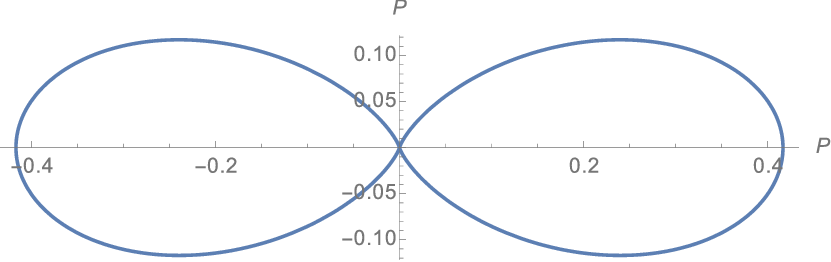
\includegraphics[width = \textwidth]{orbital-sd-polar.png}
    \end{subfigure}
    ~
    \begin{subfigure}[b]{0.45\textwidth}
        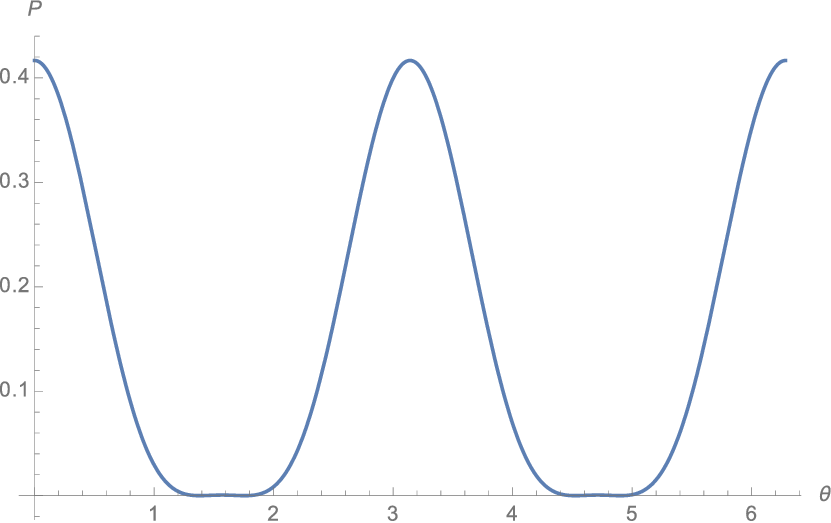
\includegraphics[width = \textwidth]{orbital-sd.png}
    \end{subfigure}
    \caption{Polar and non-polar plots of hybrid sd orbital probability densities}
    \label{fig:orbital-sd}
\end{figure}

Figures \ref{fig:orbital-sp} and \ref{fig:orbital-sd} show the probability densities of the wavefunctions, respectively. In the hybrid sp orbital, the probabilities are heavily biased towards one ``side'' (north) of the sphere, while the sd orbital has an equal balance on both ``sides'' (north and south). Additionally, probabilities only fall to zero at two points in the sp orbital, while there are four zeroes in the sd (for \(\theta \in [0, 2 \pi)\)).

\section{Using the results of the Schr\"odinger equation solved for a hydrogen-like system, calculate the difference of electron binding energies in hydrogen and in tritium. Present your answer as a formula and also give the value in \si{\electronvolt}.}
The energy levels of a hydrogen-like system are given by (found by solving the Schr\"odinger equation):
\[E_n = -\frac{\mu Z^2 e^4}{8 \epsilon_0^2 h^2 n^2}\]

The binding energy is simply how much energy it takes to excite the particle to it's ``final'' state, or \(n \to \infty\);
\[E = E_\infty - E_n = \frac{\mu Z^2 e^4}{8 \epsilon_0^2 h^2 n^2}\]

For hydrogen, we have:
\begin{align*}
    Z &= 1 \\
    \mu &= \frac{m_e m_p}{m_e + m_p} \\
    \therefore E_H &= \frac{m_e m_p}{m_e + m_p} \frac{e^4}{8 \epsilon_0^2 h^2 n^2} \\
    E_H &\big|_{n = 1} \approx \SI{13.598}{\electronvolt}
\end{align*}

For tritium, we have:
\begin{align*}
    Z &= 1 \\
    \mu &= \frac{3 m_e m_p}{m_e + 3 m_p} \\
    \therefore E_T &= \frac{3 m_e m_p}{m_e + 3 m_p} \frac{e^4}{8 \epsilon_0^2 h^2 n^2} \\
    E_T &\big|_{n = 1} \approx \SI{13.603}{\electronvolt}
\end{align*}

Thus the difference is:
\begin{align*}
    E_T - E_H &= \left(\frac{3 m_e m_p}{m_e + 3 m_p} - \frac{m_e m_p}{m_e + m_p}\right) \frac{e^4}{8 \epsilon_0^2 h^2 n^2} \\
    &\big|_{n = 1} \approx \SI{4.94}{\milli\electronvolt}
\end{align*}

\section{Find an explicit form of the velocity operator for a charged particle in a magnetic field.}
We have our Hamiltonian operator in a magnetic field:
\begin{align*}
    \hat{\mathbf{H}} &= \frac{(\hat{\mathbf{p}} - q \mathbf{A})^2}{2 m} \\
    &= \frac{1}{2 m} \left(\hat{\mathbf{p}}^2 - q ( \hat{\mathbf{p}} \cdot \mathbf{A} + \mathbf{A} \cdot \hat{\mathbf{p}}) + q^2 \mathbf{A}^2\right)
\end{align*}

As well as some ``base'' commutators:
\begin{align*}
    [\hat{\mathbf{p}}, \hat{\mathbf{r}}] &= -i \hbar \\
    [\mathbf{A}, \hat{\mathbf{r}}] &= 0 \\
    [\mathbf{A}^2, \hat{\mathbf{r}}] &= 0
\end{align*}

We can then work out the velocity operator as follows:
\begin{align*}
    \hat{\mathbf{v}} &= \frac{i}{\hbar} [\hat{\mathbf{H}}, \hat{\mathbf{r}}] \\
    &= \frac{i}{2 \hbar m} \left([\hat{\mathbf{p}}^2, \hat{\mathbf{r}}] - q([\hat{\mathbf{p}} \cdot \mathbf{A}, \hat{\mathbf{r}}] + [\mathbf{A} \cdot \hat{\mathbf{p}}, \hat{\mathbf{r}}]) + q^2 [\mathbf{A}^2, \hat{\mathbf{r}}]\right) \\
    &= \frac{i}{2 \hbar m} (\hat{\mathbf{p}} \cdot [\hat{\mathbf{p}}, \hat{\mathbf{r}}] + [\hat{\mathbf{p}}, \hat{\mathbf{r}}] \cdot \hat{\mathbf{p}} - q(\hat{\mathbf{p}} \cdot [\mathbf{A}, \hat{\mathbf{r}}] + [\hat{\mathbf{p}}, \hat{\mathbf{r}}] \cdot \mathbf{A} + \mathbf{A} \cdot [\hat{\mathbf{p}}, \hat{\mathbf{r}}] + [\mathbf{A}, \hat{\mathbf{r}}] \cdot \hat{\mathbf{p}})) \\
    &= \frac{i}{2 \hbar m} (-2 i \hbar \hat{\mathbf{p}} + 2 i \hbar q \mathbf{A}) \\
    &= \frac{1}{m} (\hat{\mathbf{p}} - q \mathbf{A})
\end{align*}

\end{document}
